
\documentclass[10pt,xcolor=table]{beamer}
\usepackage[french]{babel}
\usepackage[T1]{fontenc}
\usepackage[utf8]{inputenc}
\usetheme{Warsaw}
\usepackage{pdfpages}

\title{Outil automatique de décryptage}

\begin{document}
\begin{frame}
\begin{center}
\Huge {Outil automatique de décryptage}
\end{center}
\end{frame}


%nico
\begin{frame}
  \frametitle{Introduction}

  \begin{itemize}[<+->]
  \item La Stéganographie,
  \item Origine de la cryptographie,
  \item Ronald Rivest et le cryptage RSA
  
  \begin{block}{Les 3 critères}
    \begin{itemize}
    \item Confidentialité,
    \item Authenticité,
    \item integrité
    \end{itemize}
  \end{block}
  \end{itemize}
  \pause
  \begin{center}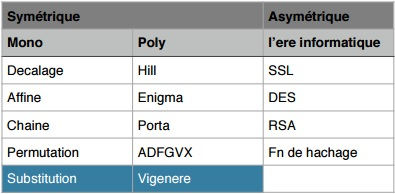
\includegraphics[scale=0.4]{Tab1.jpg}\end{center}

\end{frame}


\begin{frame}[<+->]
  \frametitle{Dcrypt}
  
  \begin{exampleblock}{Produit sur le marché}
	\begin{enumerate}
    \item www.dcode.fr,
    \item Decrypto (Google Play Store),
    \item Axcrypt
    \end{enumerate}
  \end{exampleblock}

  \begin{block}{Phase de développement}
   
    \begin{enumerate}
    \item Identification,
    \item Définition,
    \item Réalisation,
    \item Finalisation
    \end{enumerate}
  \end{block}

\end{frame}
%flo
\begin{frame}
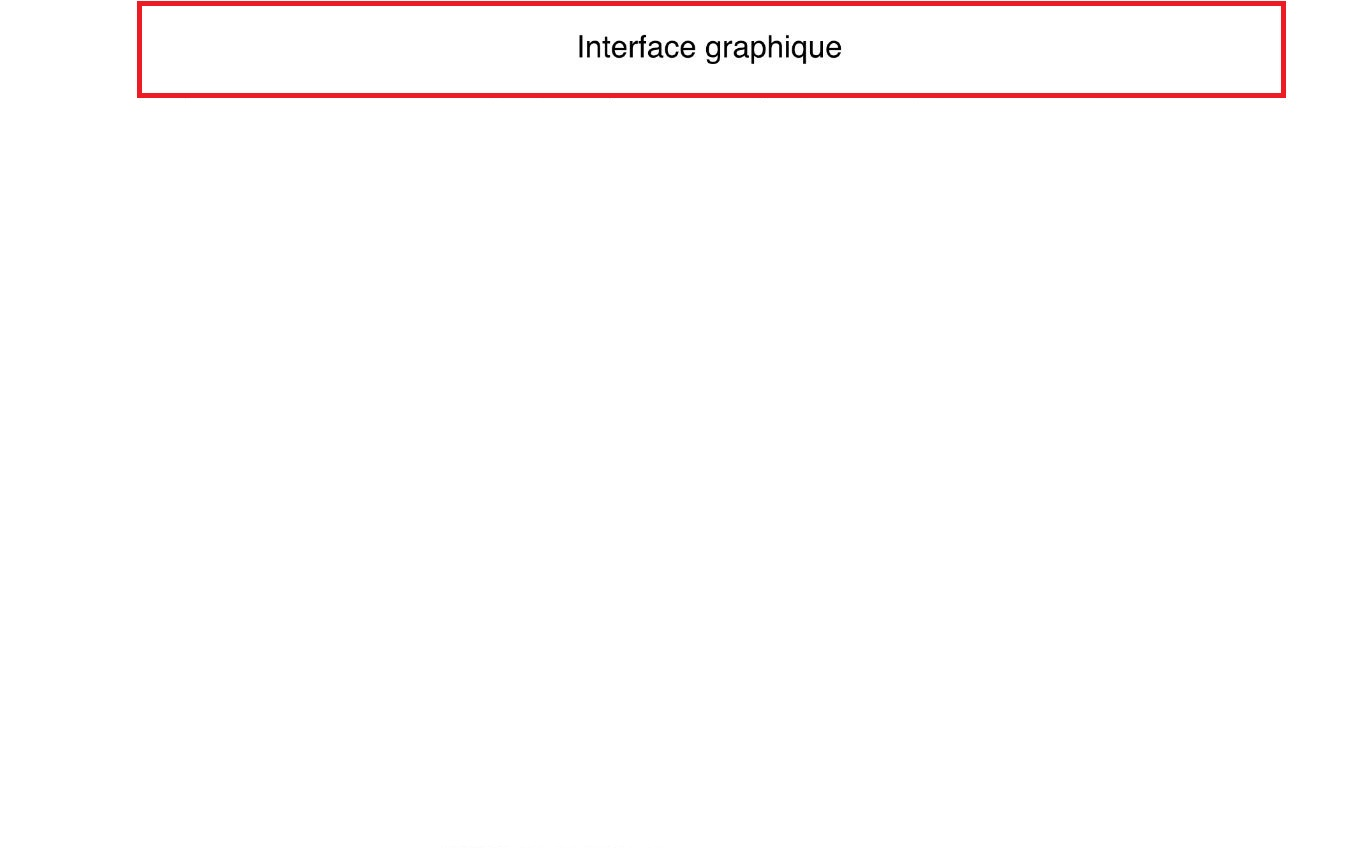
\includegraphics[scale = 0.22]{Org1.jpg}
\end{frame}
\begin{frame}
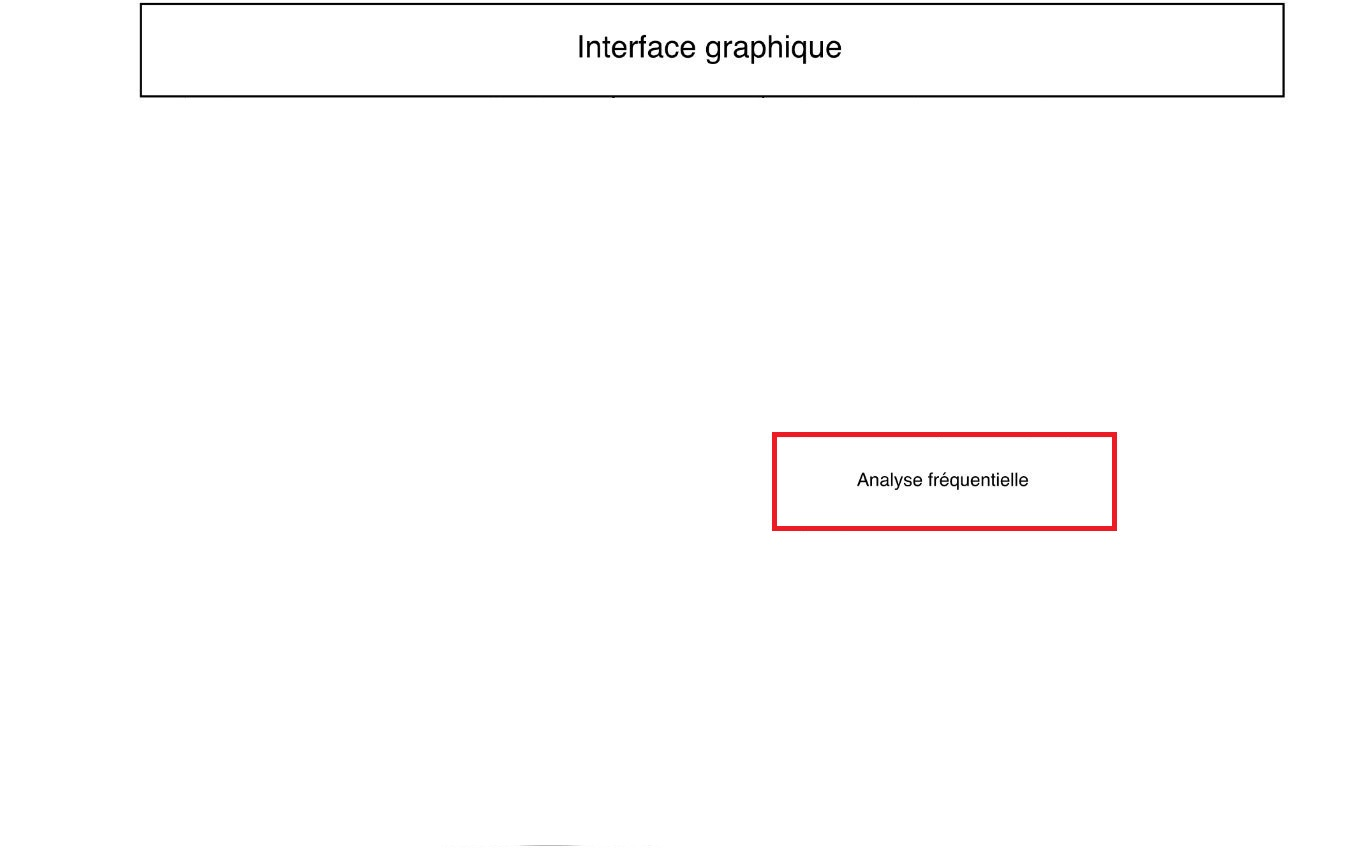
\includegraphics[scale = 0.22]{Org2.jpg}
\end{frame}
\begin{frame}
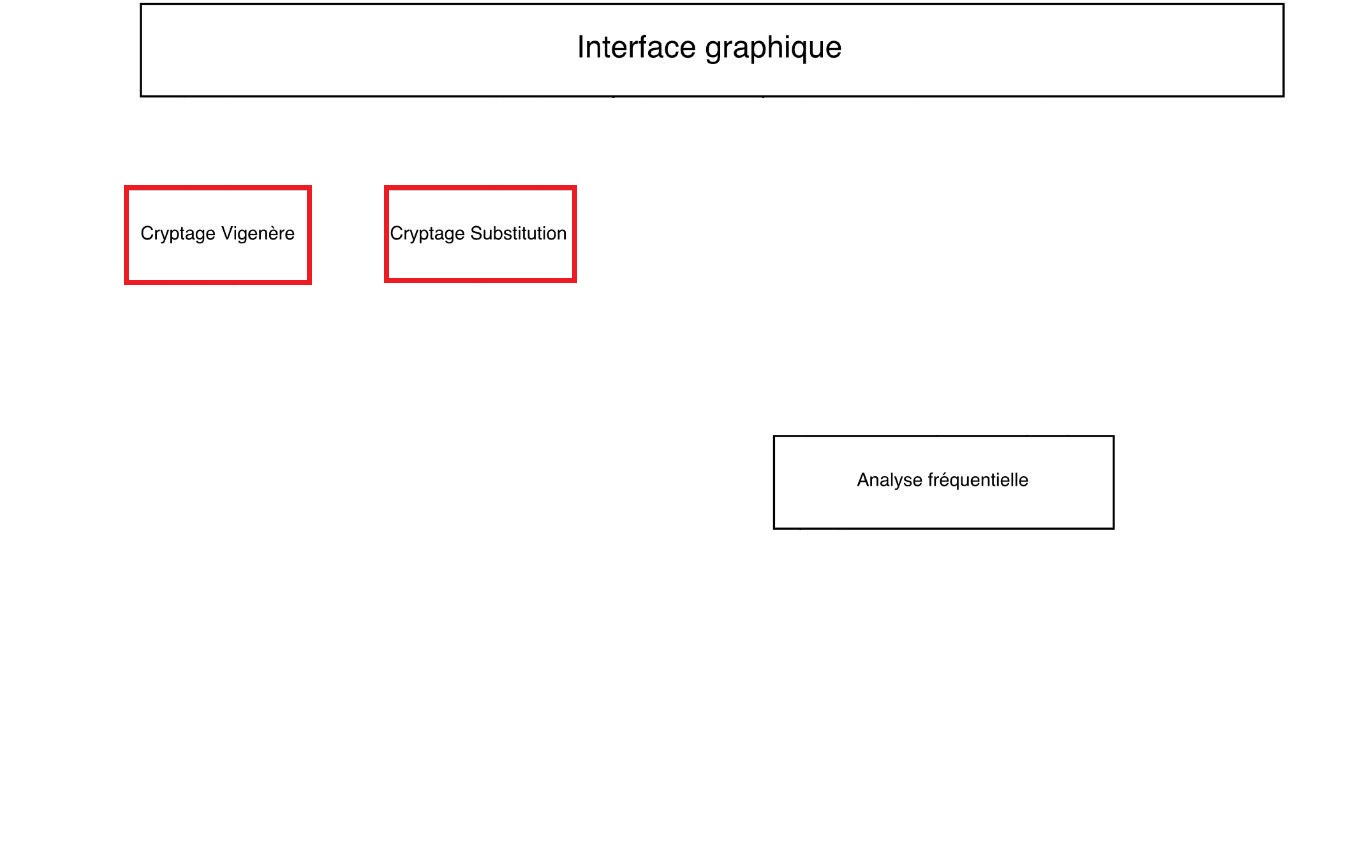
\includegraphics[scale = 0.22]{Org3.jpg}
\end{frame}
\begin{frame}
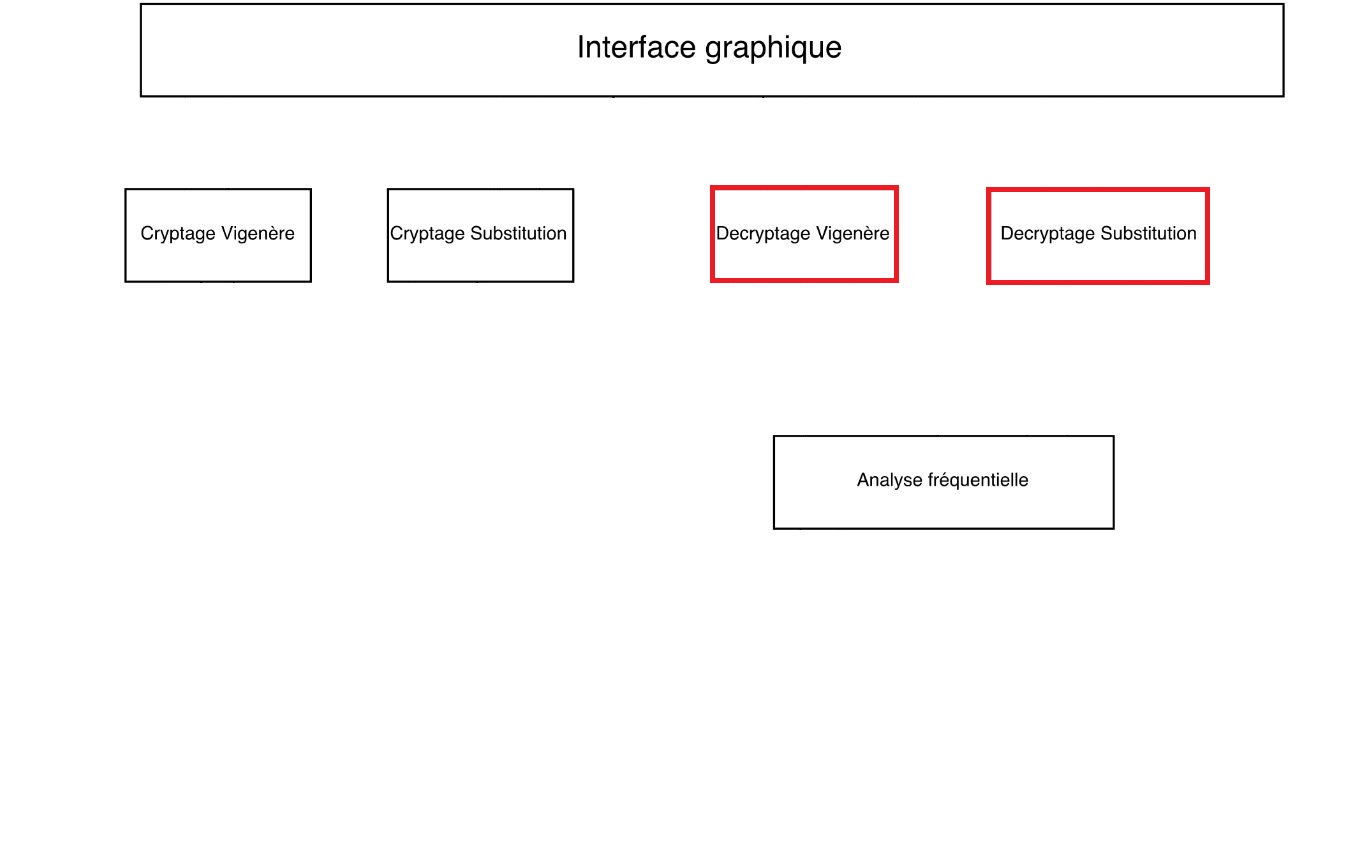
\includegraphics[scale = 0.22]{Org4.jpg}
\end{frame}
\begin{frame}
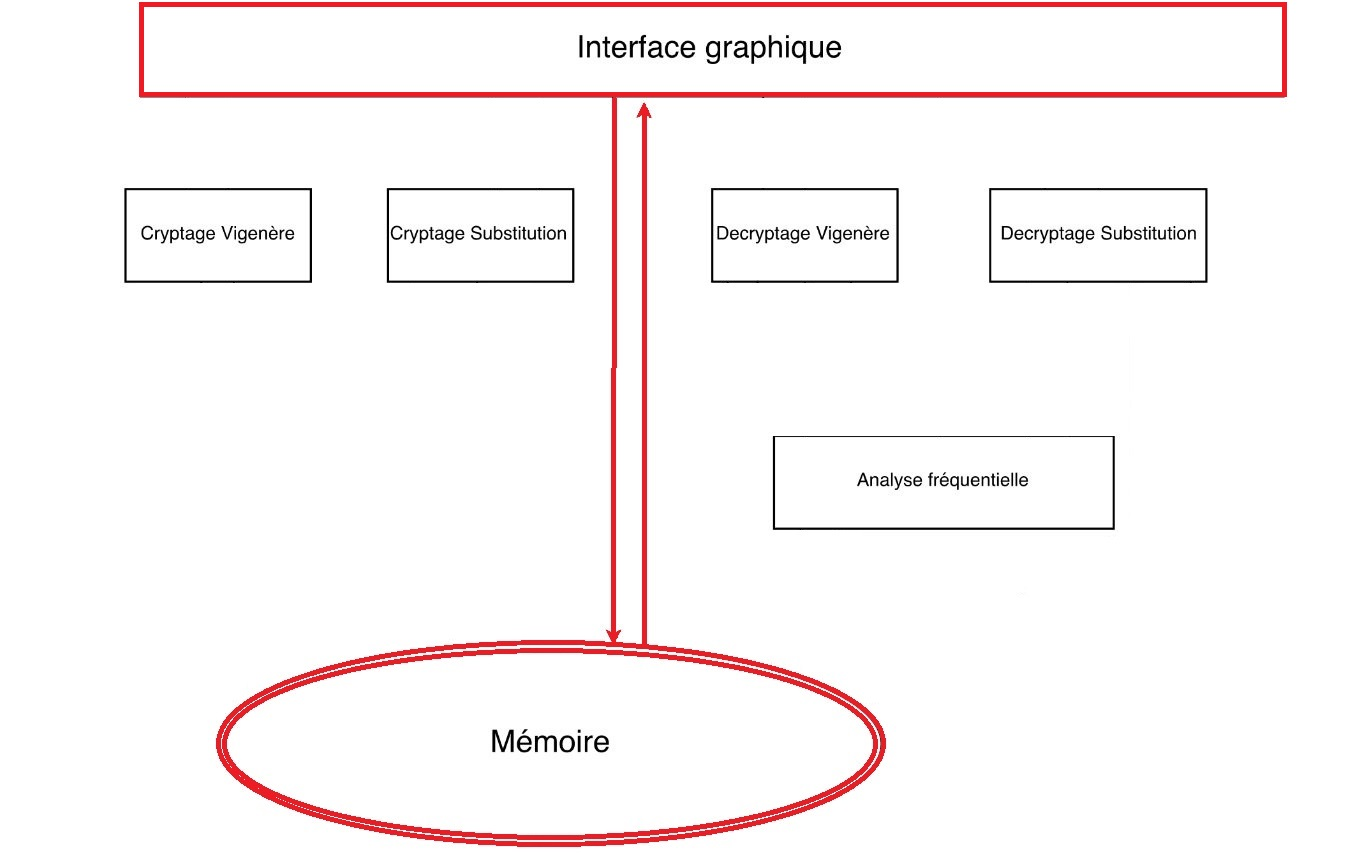
\includegraphics[scale = 0.22]{Org5.jpg}
\end{frame}
\begin{frame}
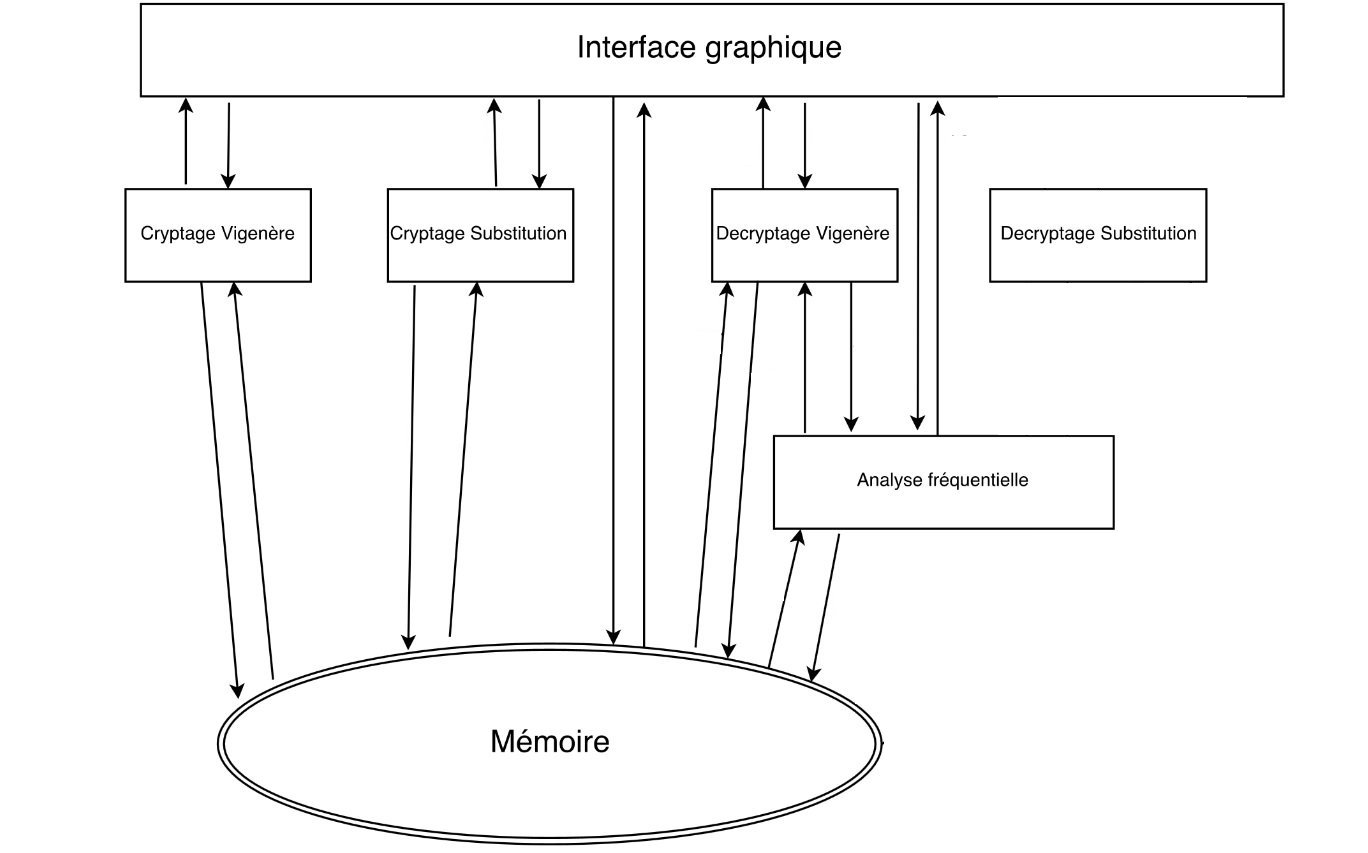
\includegraphics[scale = 0.22]{Org6.jpg}
\end{frame}
\begin{frame}
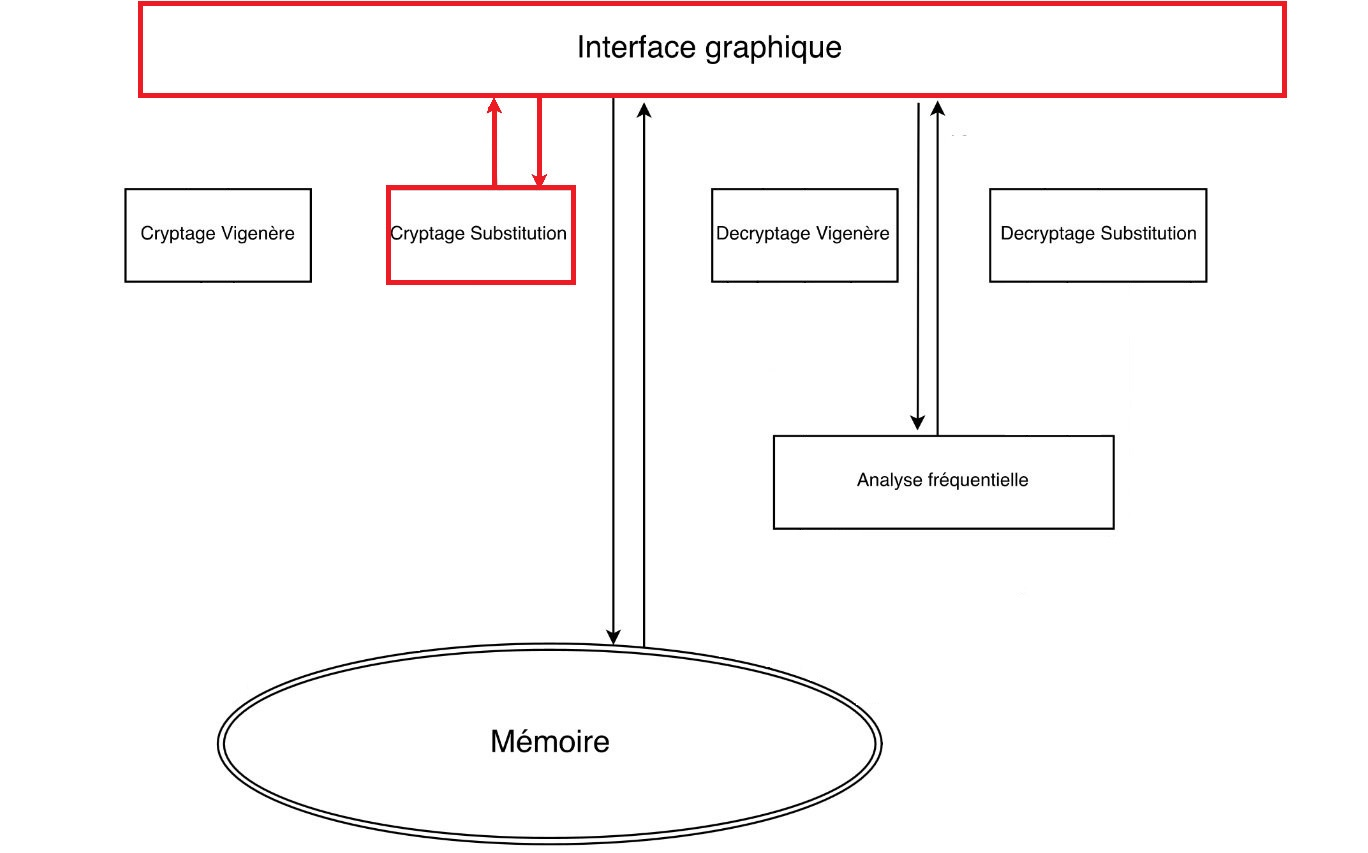
\includegraphics[scale = 0.22]{Org7.jpg}
\end{frame}
%tibo
\begin{frame}
	\begin{block}{Hypothèse du coûts en nombre de ligne}
	\begin{center}
		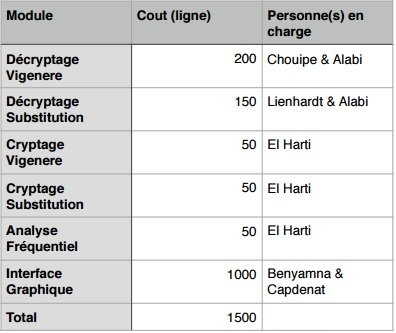
\includegraphics[scale =0.5]{Tableau_cout.jpg} \\ \pause
	\end{center}
	\end{block}
	\begin{block}{Choix du language}
	\begin{itemize}
		\item Language C \\ \pause
		\item Bibliothéque GTK +
	\end{itemize}
	\end{block}
\end{frame}
%younes
\begin{frame}
	partie technique
	\begin{block}{Interface graphique}
	\begin{itemize}
		\item passer des arguments\\ \pause
		\item switch\\ \pause
		\item seg fault de l'enregistrement
	\end{itemize}
	\end{block}
	\begin{block}{Analyse fréquentielle}
	\begin{itemize}
		\item strcpy \pause
	\end{itemize}
	\end{block}
	\begin{block}{Decryptage Vigenere}
	\begin{itemize}
		\item kasiski\\ \pause
	\end{itemize}
	\end{block}
	\begin{block}{Decryptage Substitution}
	\begin{itemize}
		\item estimations\\ \pause
	\end{itemize}
	\end{block}
\end{frame}
%zak
\begin{frame}
	\begin{block}{organisation interne}
	\end{block}
	\begin{block}{taches}
	\begin{center}
		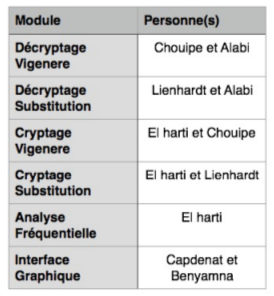
\includegraphics[scale =0.45]{taches.png} \\ 
	\end{center}
	\end{block}
\end{frame}
\begin{frame}
	\begin{block}{Planing}
	\end{block}
	\begin{block}{coûts en nombre de ligne}
	\begin{center}
		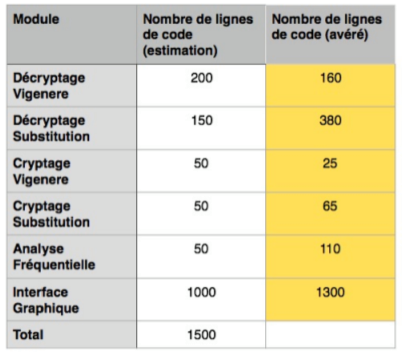
\includegraphics[scale =0.3]{tabl.png} \\ 
	\end{center}
	\end{block}
\end{frame}
%abio
\begin{frame}
\begin{center}
\Huge {Conclusion}\pause
\end{center}
\begin{center}

\includegraphics[scale =0.5]{logo.png}
\end{center}
\end{frame}


\end{document}
